\subsection*{Opgave 1}

For en standardnormalfordelt stokastisk variabel ($\mu = 0$ og $\sigma = 1$) bestem da følgende sandsynligheder.

\begin{enumerate}[label=\roman*)]
	\item Sandsynligheden for at få et udfald inden for én spredning fra middelværdien.
	\item Sandsynligheden for at få et udfald inden for to spredninger fra middelværdien.
	\item Sandsynligheden for at få et udfald inden for tre spredninger fra middelværdien.
	\item Sandsynligheden for at få et normalt udfald.
	\item Sandsynligheden for at få et exceptionelt udfald.
\end{enumerate}



\subsection*{Opgave 2 (Uden Maple)}
	Af Fig. \ref{fig:fordeling} ses fordelingsfunktionerne $F$ og $G$ for to normalfordelte stokastiske variable
	\begin{align*}
		X \sim N(\mu,1)
	\end{align*}
	og 
	\begin{align*}
		Y \sim N(\mu,1.5).
	\end{align*}
	\begin{figure}[H]
		\centering
		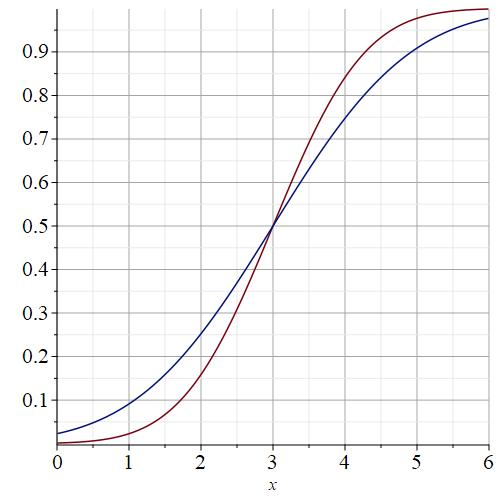
\includegraphics[width=0.7\textwidth]{Billeder/fordelingafl.jpg}
		\caption{Fordelingsfunktionerne $F$ og $G$.}
		\label{fig:fordeling}
	\end{figure}
\begin{enumerate}[label=\roman*)]
	\item Bestem middelværdien $\mu$ for de to stokastiske variable.
	\item Hvilken af de to kurver tilsvarer fordelingsfunktionen for henholdsvis $X$ og $Y$?
	\item Bestem sandsynlighederne
		\begin{align*}
			P(2<X<4) \textnormal{ og } P(1<Y).
		\end{align*}
\end{enumerate}


\subsection*{Opgave 3}

I Opgave 1 ii) er I formentlig kommet frem til, at det ikke giver et nøjagtigt 95$\%$- konfidensinterval at ligge 2 spredninger fra middelværdien som vi jo anvendte, da I lavede konfidensintervaller i forbindelse med binomialtest. 
\begin{enumerate}[label=\roman*)]
	\item Hvor mange spredninger skal vi ligge fra middelværdien for at få et (mere) nøjagtigt
	$95\%$-konfidensinterval?
\end{enumerate}

\subsection*{Opgave 4}

Vægten af en pose med lakridser antages at være normalfordelt med $\mu = 200$g og $\sigma = 4.2$g.

\begin{enumerate}[label=\roman*)]
	\item Hvilke af udfaldene 205g, 211g, 189g og 186g er normale og hvilke er exceptionelle?
	\item Hvad er z-værdien for udfaldene 185g, 201g og 213g?
\end{enumerate}

\subsection*{Opgave 5}


	\begin{center}
		\includegraphics[width=0.7\textwidth]{Billeder/choko.jpg}
	\end{center}
	En producent af chokoladebarer har undersøgt en bestemt slags af sine chokoladebarer og opdaget, at vægten af netop dén type chokoladebar er normalfordelt
	med en middelværdi på 51g og en spredning på 4.5g.
\begin{enumerate}[label=\roman*)]
	\item Afgør, om en chokoladebar på 57g er et normalt udfald. 
\end{enumerate}

	
Vi lader $f$ betegne tæthedsfunktionen for den normalfordelte stokastiske variabel, der beskriver vægten af chokoladebarerne. 
\begin{enumerate}[label=\roman*)]
	\setcounter{enumi}{1}
	\item Hvad siger følgende integral om vægten af chokoladebarerne?
	\begin{align*}
		\int_{48}^{65} f(x)dx \approx  0.747.
	\end{align*}
\end{enumerate}

\subsection*{Opgave 6}

Om en normalfordelt stokastisk variabel med $\mu = 12$ og tæthedsfunktion $f$ gælder det, at
\begin{align*}
	\int_9^{15} f(x) \intd x \approx 68.3.
\end{align*}
	
\begin{enumerate}[label = \roman*)]
	\item Bestem spredningen for $X$. 
	\item Bestem $a$, så $P(12 - a < X < 12 + a) = 0.8$. 
	\item Bestem $b$, så $P(X < b) = 0.997$. 
\end{enumerate}

\subsection*{Opgave 7}

En stokastisk variabel $X$ har tæthedsfunktion

\begin{align*}
	f(x) = \frac{1}{\sqrt{2\pi}3}e^{-\frac{1}{2}\left(\frac{x-67}{3}\right)^2}.
\end{align*}

\begin{enumerate}[label = \roman*)]
	\item Aflæs middelværdien og spredningen for $X$.
	\item Bestem sandsynligheden $P(65 < X)$.
	\item Bestem $a$, så 
	\begin{align*}
		\int_a^{70} f(x) \intd x = 0.79.
	\end{align*}
	\item Bestem $z$-værdien for udfaldet 60.
\end{enumerate}

